\documentclass{beamer}
\usetheme{Madrid}
\usecolortheme{seahorse}

\usepackage{graphicx}
\usepackage{listings}
\usepackage{booktabs}

\title[Greenhouse Gas Emission Extraction]{Extracting Greenhouse Gas Emission Values from Corporate Sustainability Reports}
\subtitle{A Case Study on Evaluating and Finetuning Language Models on Long-Context Structured Information Extraction}
\author{}
\date{March 11, 2024}
\begin{document}
\begin{frame}[plain]
    \maketitle
    \url{https://github.com/nopperl/corporate_emission_reports}
\end{frame}
\begin{frame}{Motivation}

\begin{block}{Current State}
	\begin{itemize}
		\item Data about corporate greenhouse gas (GHG) emissions is usually published only as part of sustainability report \alert{PDF files}.
		\item This format is not \alert{machine-readable}.
		\item Interested actors have to manually extract emission data from these reports.
		\item This process is \alert{tedious} and \alert{time-consuming}.
	\end{itemize}
\end{block}

\begin{block}{Potential Solution}
	An automatic information-extraction system could:
	\begin{itemize}
		\item Extract GHG emissions data from sustainability report PDF files.
		\item Provide the data in a machine-readable format.
		\item Save time and effort for interested actors.
	\end{itemize}
\end{block}
\end{frame}

%\begin{frame}{Objective}
%\begin{itemize}
%	\item Open source system that extracts Scope 1, 2 and 3 greenhouse gas (GHG) emissions in metric tonnes
%	of CO2eq in a machine-readable format from sustainability reports.
%	\item Definitions based on  \begin{itemize}
%			\item Scope 1: A reporting organization’s direct GHG emissions.
%		\item Scope 2: A reporting organization’s emissions associated with the generation of electricity, heating/cooling, or steam purchased for own consumption.
%		\item Scope 3: A reporting organization’s indirect emissions other than those covered in scope 2.
%		\end{itemize}
%		
%	\item Also indicates the pages in the report containing GHG emission values.
%\end{itemize}
%\end{frame}

\begin{frame}[fragile=singleslide]{Objective}{Example}
	

	\begin{block}{Example input (excerpt)}
   \begin{figure}[h]
	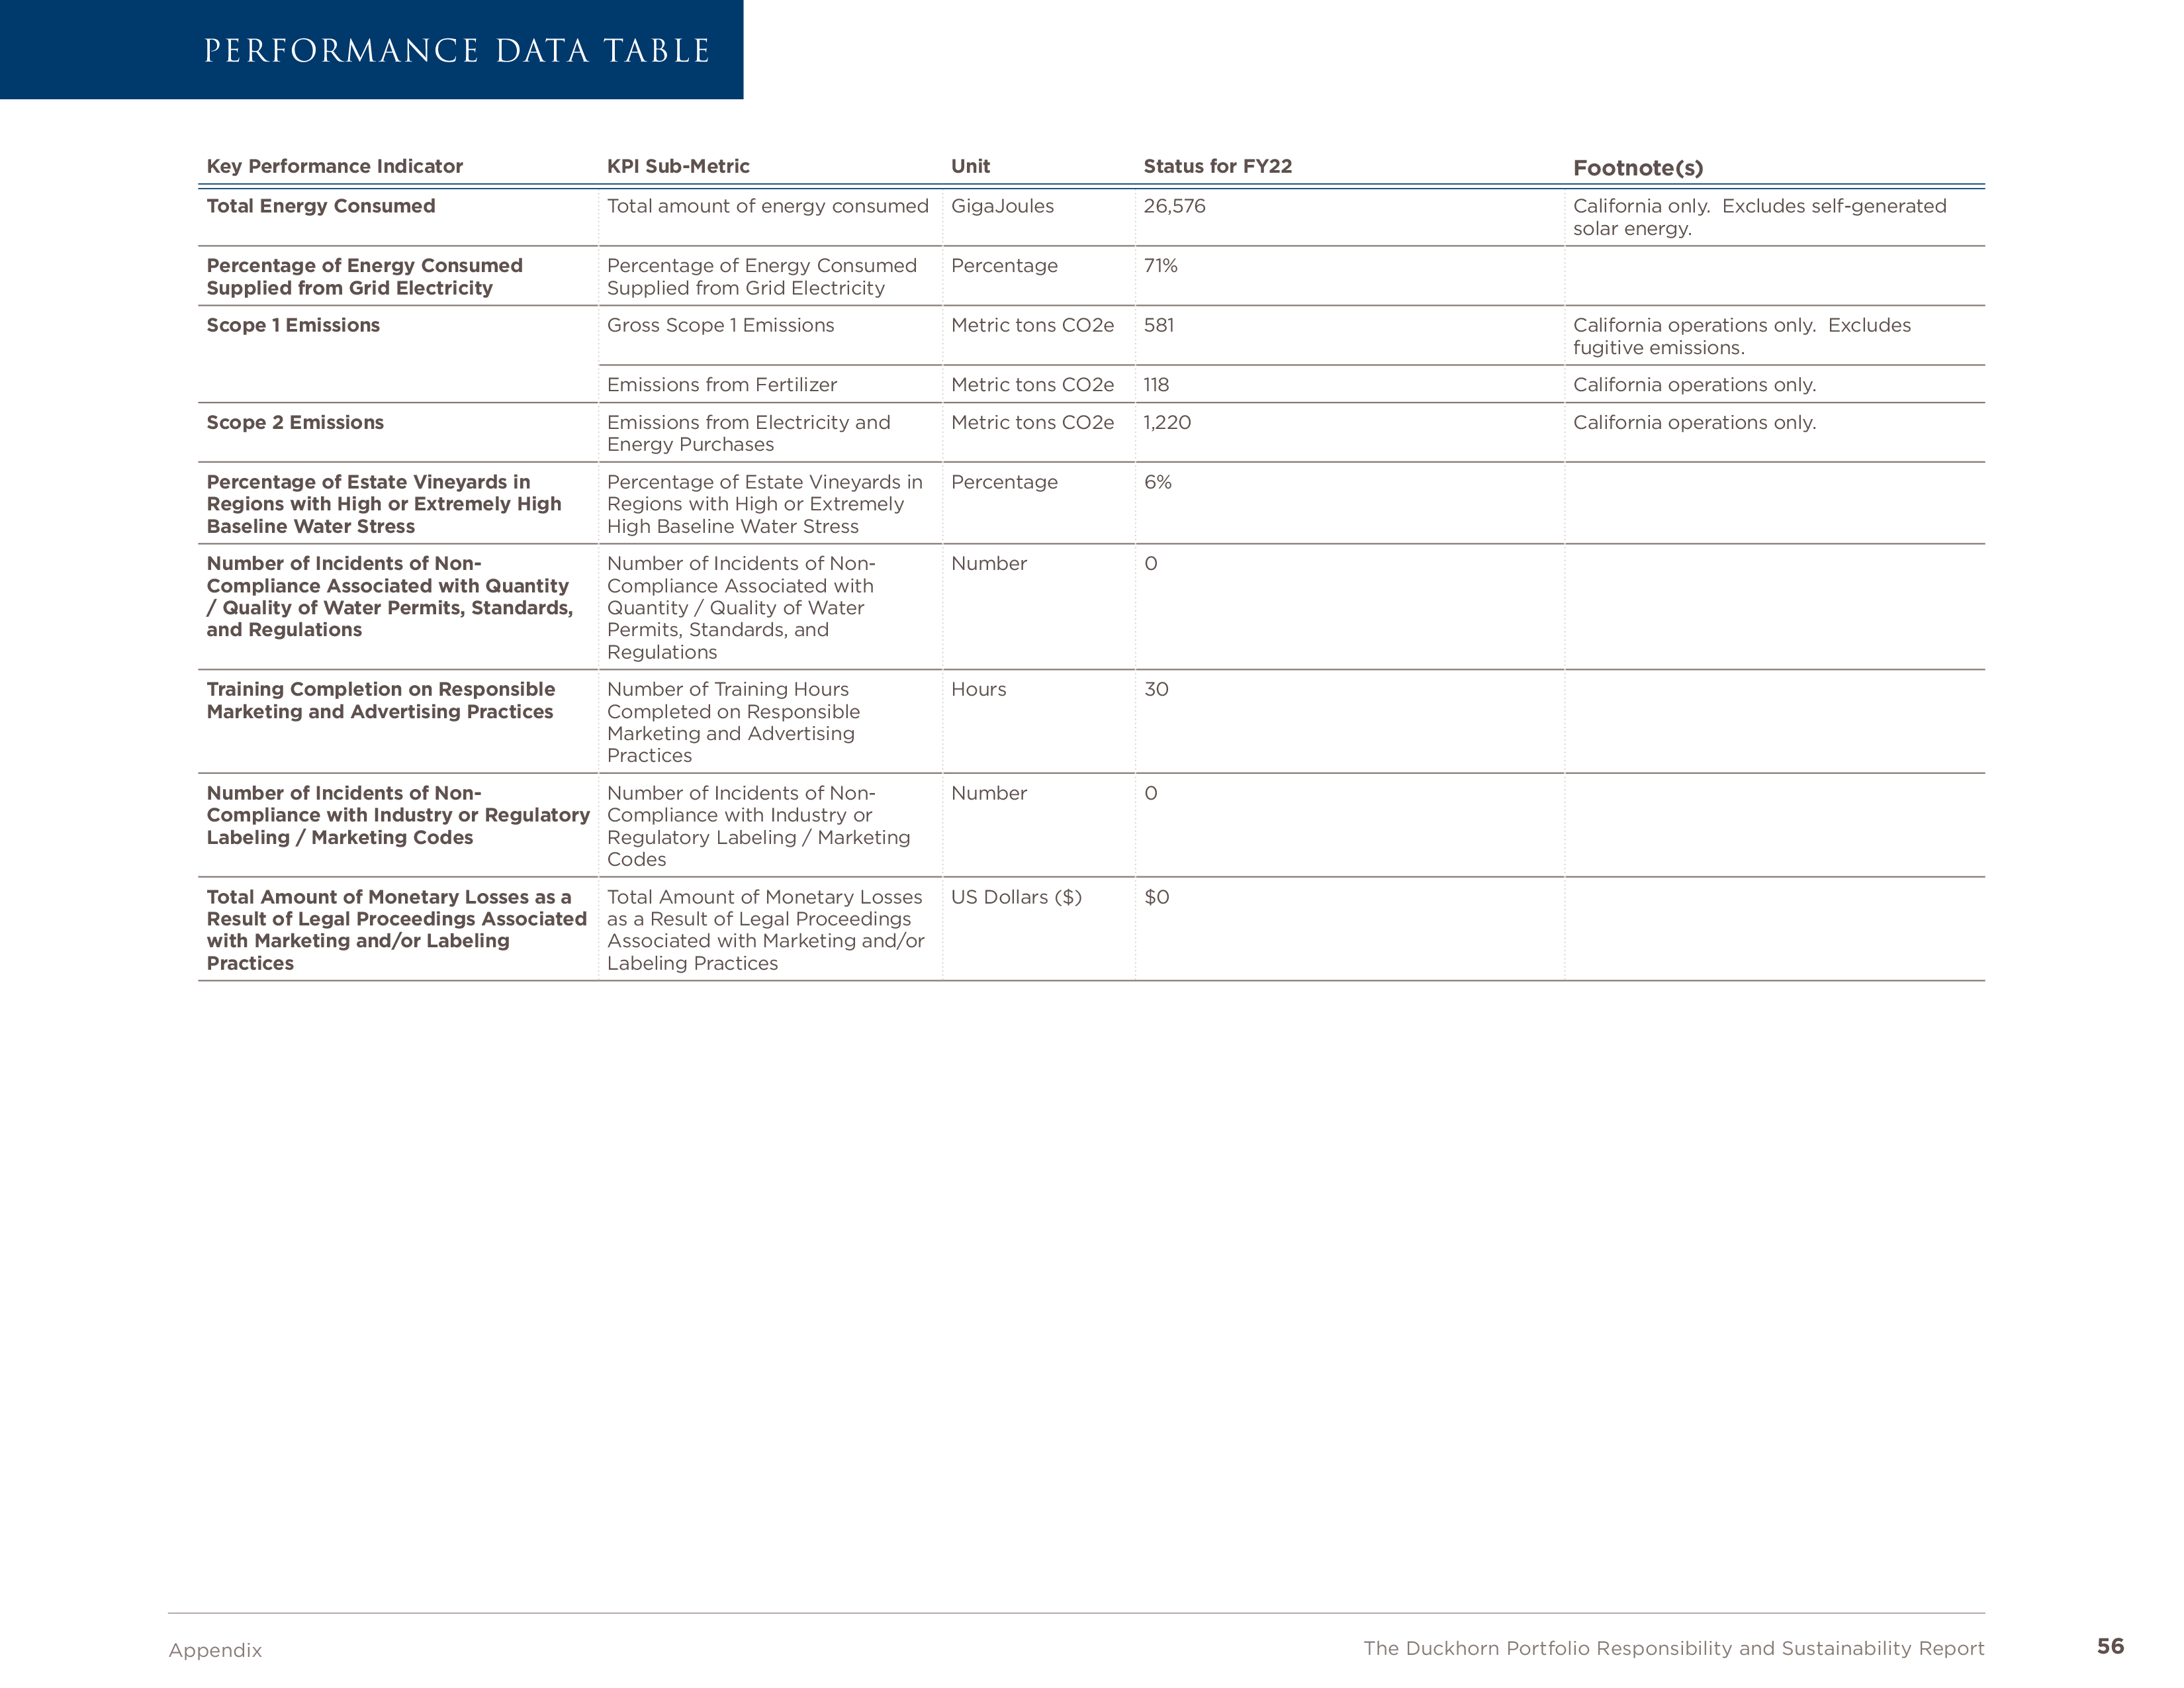
\includegraphics[width=\textwidth, trim={0 {5\textheight} 0 0}, clip]{graphics/example-report-page}
%	\caption{Relevant emission page of the 2022 sustainability report by The Duckhorn Portfolio, Inc.}
%	\label{fig:example.report.page}
\end{figure}
\end{block}
	\begin{block}{Example output}
	\tiny
	\begin{lstlisting}
{"scope_1":581,"scope_2":1220,"scope_3":null,"sources":[16,17,56,7]}
	\end{lstlisting}
\end{block}

\end{frame}

\begin{frame}{Challenges}

\begin{itemize}
\item Reports are very long $\rightarrow$ long context task.
\item No available ground truth dataset of reports and extracted GHG emission values.
\end{itemize}
\end{frame}

\begin{frame}{Approach}
	\begin{enumerate}
\item Assemble evaluation dataset.
\item Develop inference system to use language models for emission extraction.
\item Benchmark the performance of selected language models.
\item Generate finetuning dataset using best-performing large model.
\item Finetune the best-performing small model on the generated dataset.
\item Deploy the finetuned model.
	\end{enumerate}
\end{frame}

\begin{frame}{Evaluation dataset}
\begin{itemize}
\item 100 sustainability reports from geographically-diverse corporations and manually-extracted emission values.
\end{itemize}
\end{frame}

\begin{frame}{System architecture}
\begin{itemize}
\item Developed in Python.
\item Inference using llama.cpp.
\item Consists of four parts:
\begin{itemize}
\item \alert{Input data} is extracted from a sustainability report,
\item inserted into a \alert{prompt},
\item whis is used by the \alert{language model}
\item to produce a \alert{structured output}.
\end{itemize}
\end{itemize}
\end{frame}

\begin{frame}{Input data and prompt}

Simple RAG setup:

\begin{enumerate}
\item Plain-text semi-structured XHTML representation of report PDF is extracted using PyMuPDF.
\item Extracted text is split into chunks by page.
\item All chunks containing relevant GHG emission terms (such as \texttt{Scope 1}) are retrieved.
\item Retrieved plain-text chunks are inserted into a predefined prompt.
\end{enumerate}
Resulting prompt length in tokens:
\begin{table}[h]
	\begin{tabular}{lrrrr}
\toprule
 & max & mean & median & min \\
\midrule
token\_length & 60063.00 & 14544.31 & 12184.50 & 1004.00 \\
\bottomrule
\end{tabular}

\end{table}
\end{frame}

\begin{frame}[fragile=singleslide]{Output}
\begin{itemize}
\item Model output is constrained using BNF grammar to produce a JSON according to a predefined schema.
\end{itemize}
\begin{block}{Example output}
\tiny
\begin{lstlisting}
{"scope_1":581,"scope_2":1220,"scope_3":null,"sources":[16,17,56,7]}
\end{lstlisting}
\end{block}
\end{frame}

\begin{frame}{Evaluation}{Models}
\begin{table}[]
	\begin{tabular}{|l|c|c|}
		\hline
		\textbf{Model} & \textbf{Param Size} & \textbf{Context Length} \\ \hline
		\href{https://huggingface.co/mistralai/Mistral-7B-Instruct-v0.2}{Mistral-7B-Instruct-v0.2} & 7B & 32768 \\ \hline
		\href{https://huggingface.co/openchat/openchat-3.5-0106}{openchat-3.5-0106} & 7B & 8192 \\ \hline
		\href{https://huggingface.co/Qwen/Qwen-1_8B-Chat}{Qwen-1.8B-Chat} & 1.8B & 8192 \\ \hline
		\href{https://huggingface.co/mistralai/Mixtral-8x7B-Instruct-v0.1}{Mixtral-8x7B-Instruct-v0.1} & 45B & 32768 \\ \hline
		\href{https://huggingface.co/miqudev/miqu-1-70b}{miqu-1-70b} & 70B & 32764 \\ \hline
	\end{tabular}
\end{table}
Note: \texttt{Q5\_K\_M} quantization format of Mixtral-8x7B-Instruct-v0.1 and miqu-1-70b are used due to constrained resources.
\end{frame}
\begin{frame}{Evaluation}{Metrics}
\begin{enumerate}
\item accuracy for every extracted emission value
\item source page retrieval accuracy
\end{enumerate}
\end{frame}
\begin{frame}{Evaluation}{Result}
\begin{table}[h]
	\centering
	\begin{tabular}{|c|c|c|c|c|c|}
		\hline
		\textbf{scope 1} & \textbf{scope 2} & \textbf{scope 3} & \textbf{avg of scopes} & \textbf{sources} & \textbf{model} \\
		\hline
		49 & 34 & 54 & 46 & 53 & mistral \\
		33 & 31 & 56 & 40 & 48 & openchat \\
		12 & 8 & 5 & 8 & 3 & qwen-1.8B \\
		69 & 72 & 57 & 66 & 74 & miqu \\
		70 & 71 & 69 & 69 & 64 & mixtral \\
		\hline
	\end{tabular}
\end{table}
\end{frame}
\begin{frame}{Finetuning}{Dataset}
\begin{itemize}
\item Collect 3233 sustainability reports different from the evaluation dataset.
\item Generate outputs using Mixtral-8x7B-Instruct-v0.1 (the best performing model).
\item Convert into instruction format.
\end{itemize}
\end{frame}

\begin{frame}{Finetuning}{Setup}
\begin{itemize}
\item Finetune Mistral-7B-Instruct-v0.2 (the best performing $\leq$7B model).
\item axolotl is used as finetuning framework.
\item Finetuning a 7B model is resource intensive, especially for long sequences.
\item Using standard configuration, only sequences up to a length of 6144 tokens can be trained.
\item To enable training on sequences of up to 32768 tokens, following techniques are used:
\begin{itemize}
\item LoRA
\item Flash Attention 2
\item ZeRO-3
\item bfloat16
\item bitsandbytes 8-bit AdamW optimizer.
\end{itemize}
\end{itemize}
\end{frame}

\begin{frame}{Finetuning}{Evaluation}
\begin{table}[h]
	\centering
	\begin{tabular}{|c|c|c|c|c|c|}
		\hline
		\textbf{scope 1} & \textbf{scope 2} & \textbf{scope 3} & \textbf{avg of scopes} & \textbf{sources} & \textbf{model} \\
		\hline
		49 & 34 & 54 & 46 & 53 & mistral \\
		69 & 72 & 57 & 66 & 74 & miqu \\
		70 & 71 & 69 & 69 & 64 & mixtral \\
		65 & 62 & 69 & 65 & 77 & \textbf{lora} \\
		\hline
	\end{tabular}
\end{table}
\end{frame}

\begin{frame}{Contributions}
	\begin{itemize}
		\item A manually-created evaluation dataset ($N=100$),
		\item a synthetic finetuning dataset ($N=3233$),
		\item an evaluation of multiple models (1.8B-45B) covering prompt strategies, numerical issues and self extend,
		\item an evaluation of different finetuning configurations,
		\item a finetuned Mistral-7B model which nearly matches and partially exceeds Mixtral (45B) on this task, and
		\item a web demo (\url{https://huggingface.co/spaces/nopperl/emission-extractor}).
	\end{itemize}
	Source code: \url{https://github.com/nopperl/corporate_emission_reports}
\end{frame}

\begin{frame}{Future work}
\begin{itemize}
	\item Evaluate multimodal vision-language models such as CogVLM for understanding visual information in PDF documents.
	\item Improve prompts using few-shot or chain-of-thought prompting (though token-expensive).
	\item Consider testing smaller encoder(-decoder) models such as XLM-RoBERTa or DeBERTa.
\end{itemize}
\end{frame}

\end{document}
